\newcommand{\study}[1]{
\newif\ifhiggs

\IfFileExists{abc.tex}{\higgstrue}{\higgsfalse}
\ifhiggs
  \loop
  \begin{frame}
  \repeat
\fi
}
% if 
\newcommand{\widP}{1.5in}
\newcommand{\widF}{2.5in}
\newcommand{\simu}{one}
%
\newcommand{\polycube}{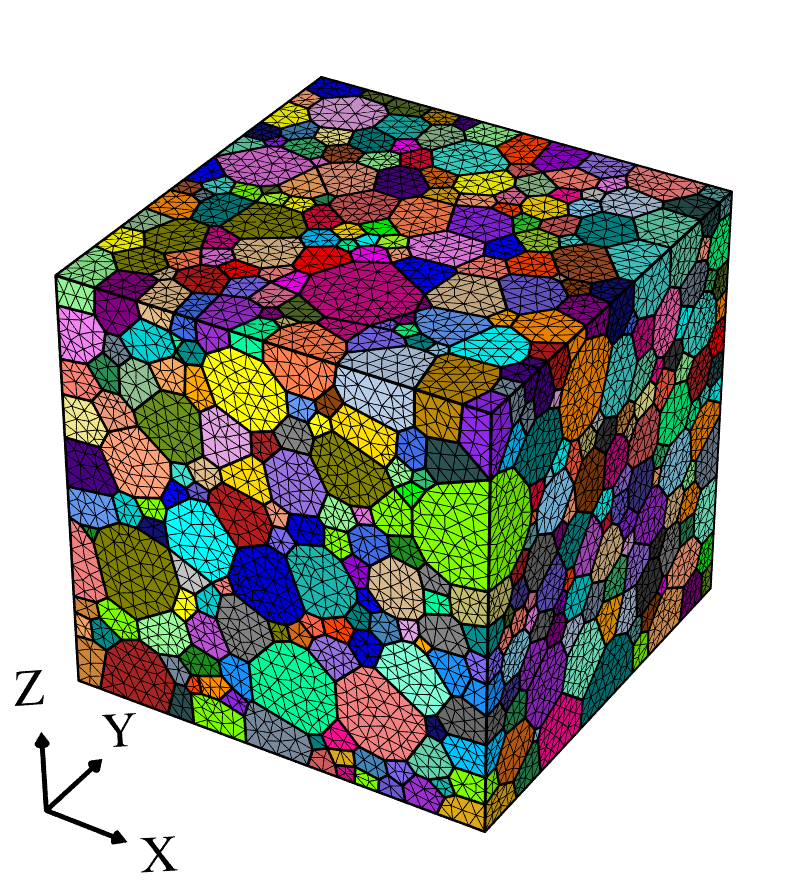
\includegraphics[width=\widP]{figures/cubic_domain.png}}
\newcommand{\polyelongated}{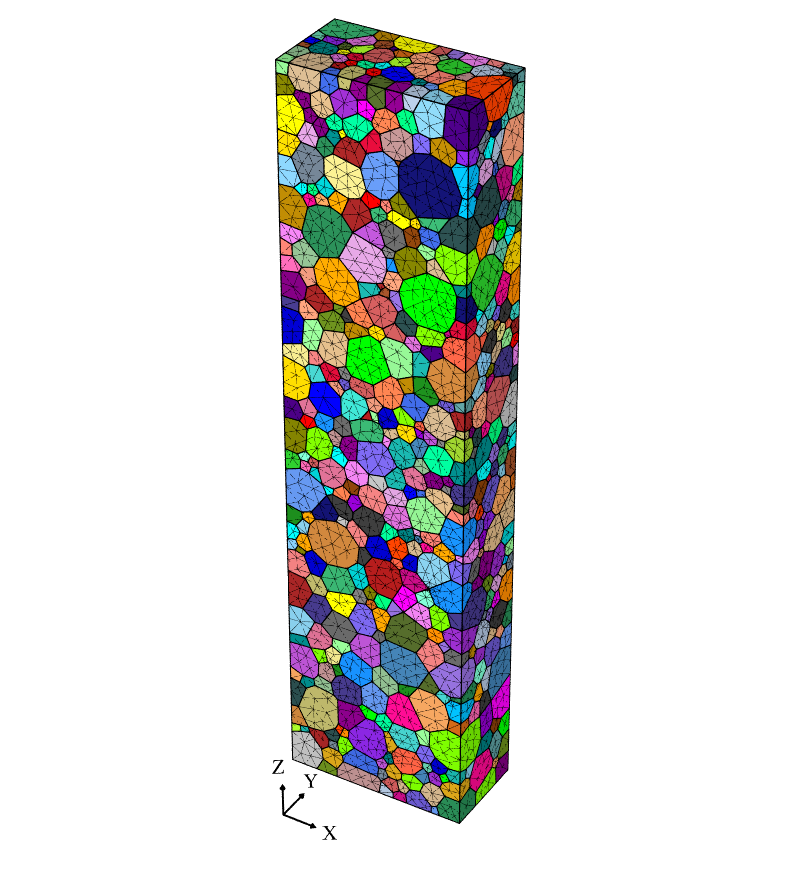
\includegraphics[width=\widP]{figures/elongated_domain.png}}
%
\newcommand{\cTimesOTF}[2]{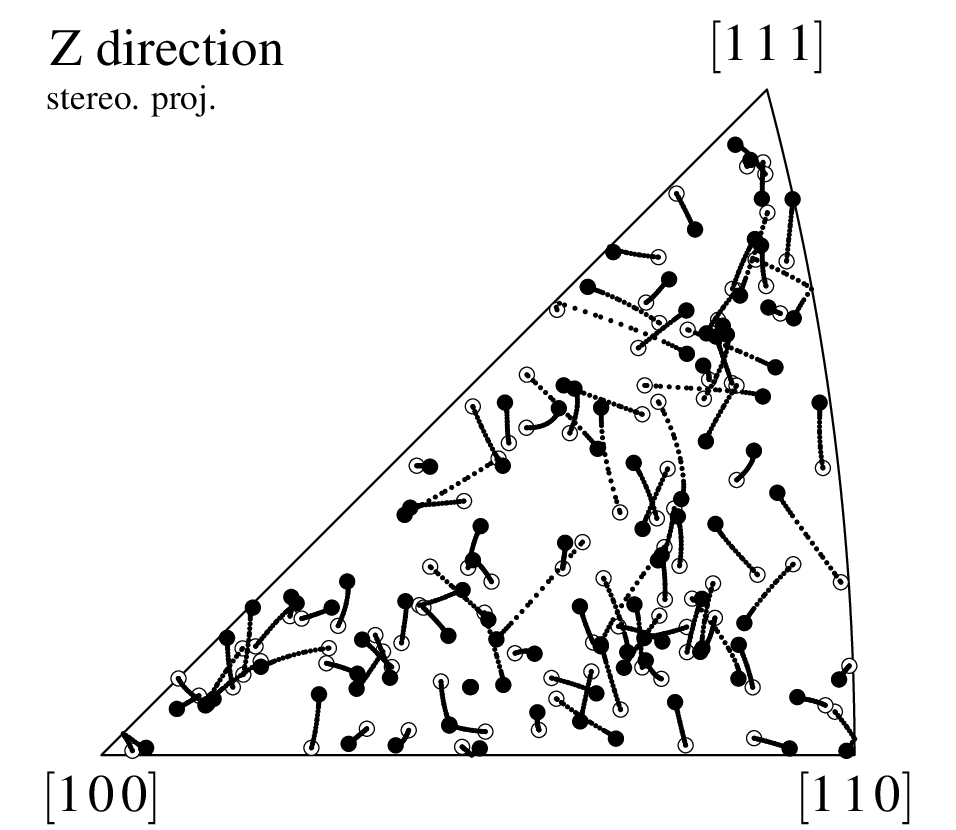
\includegraphics[width=\widF]{figures/testing_fig.png}}
\newcommand{\cTimesOFO}[2]{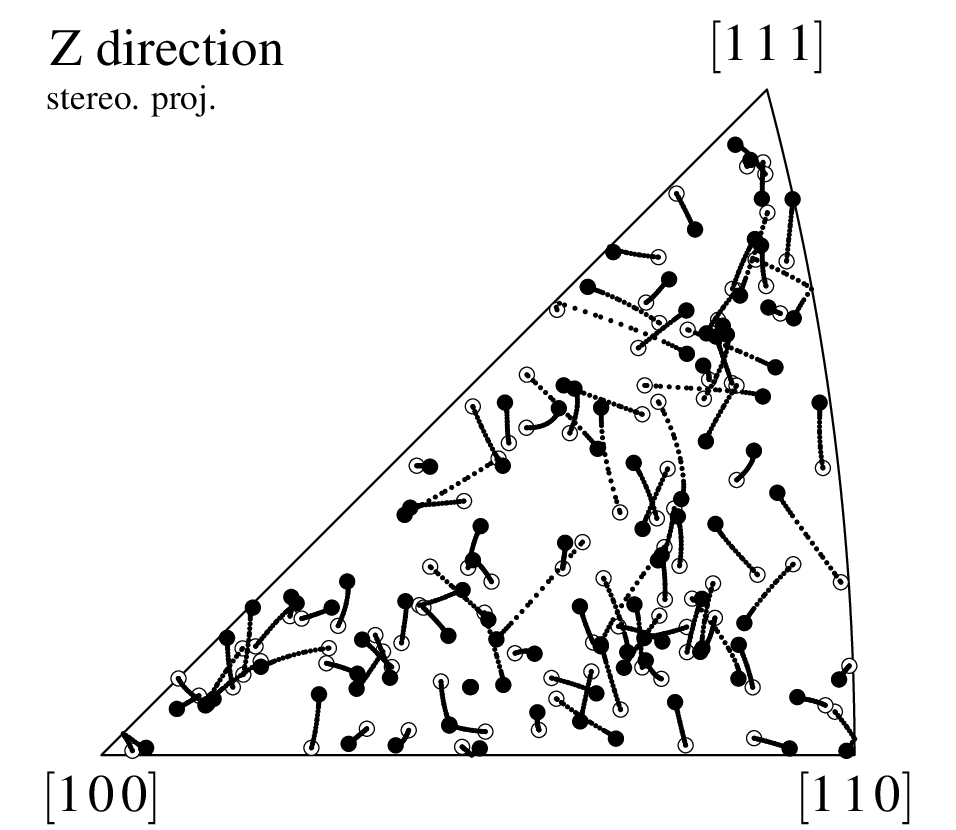
\includegraphics[width=\widF]{figures/testing_fig.png}}
\newcommand{\cTimesOSF}[2]{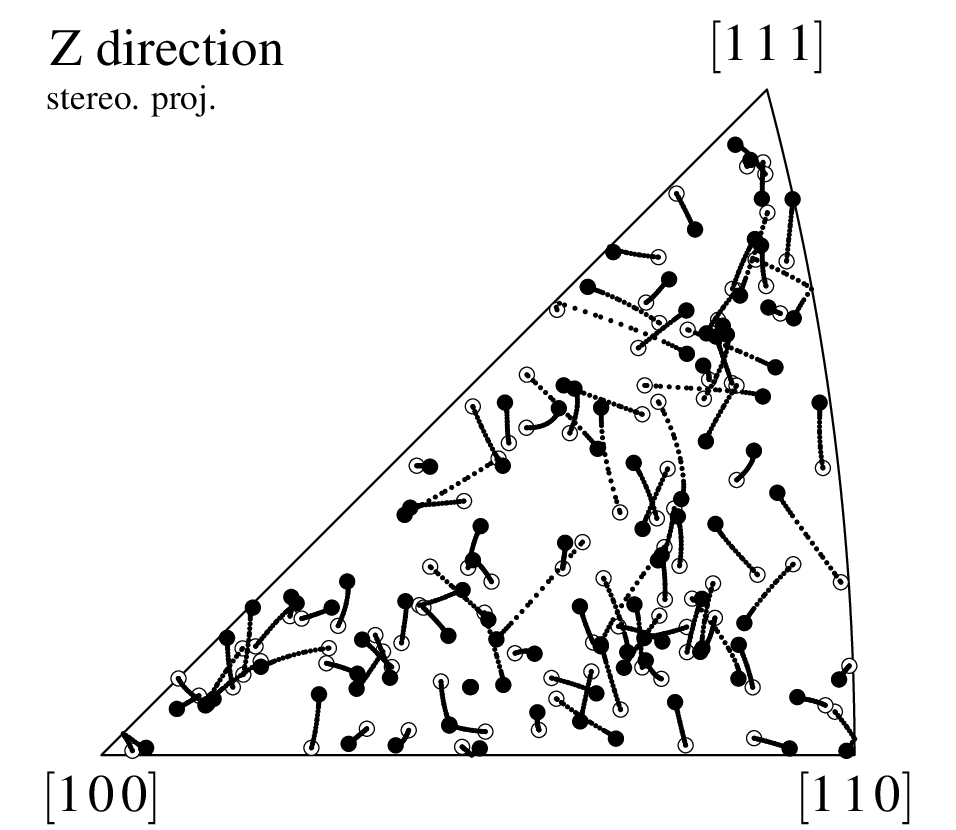
\includegraphics[width=\widF]{figures/testing_fig.png}}
\newcommand{\cTimesTH }[2]{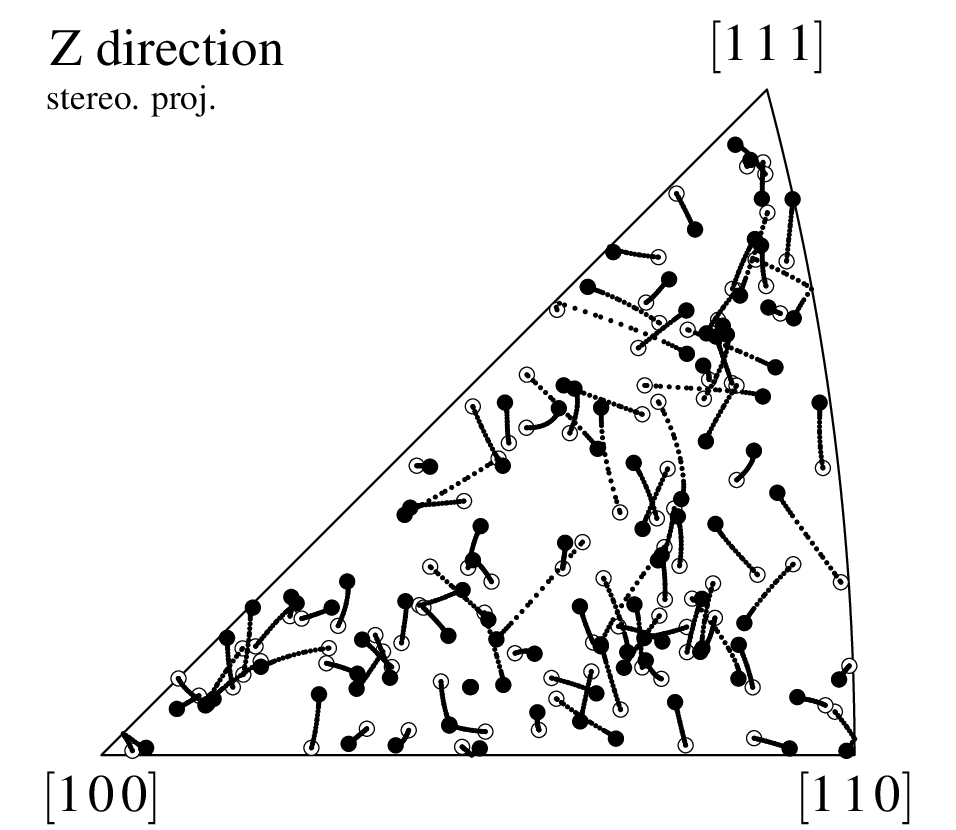
\includegraphics[width=\widF]{figures/testing_fig.png}}
\newcommand{\cTimesFH }[2]{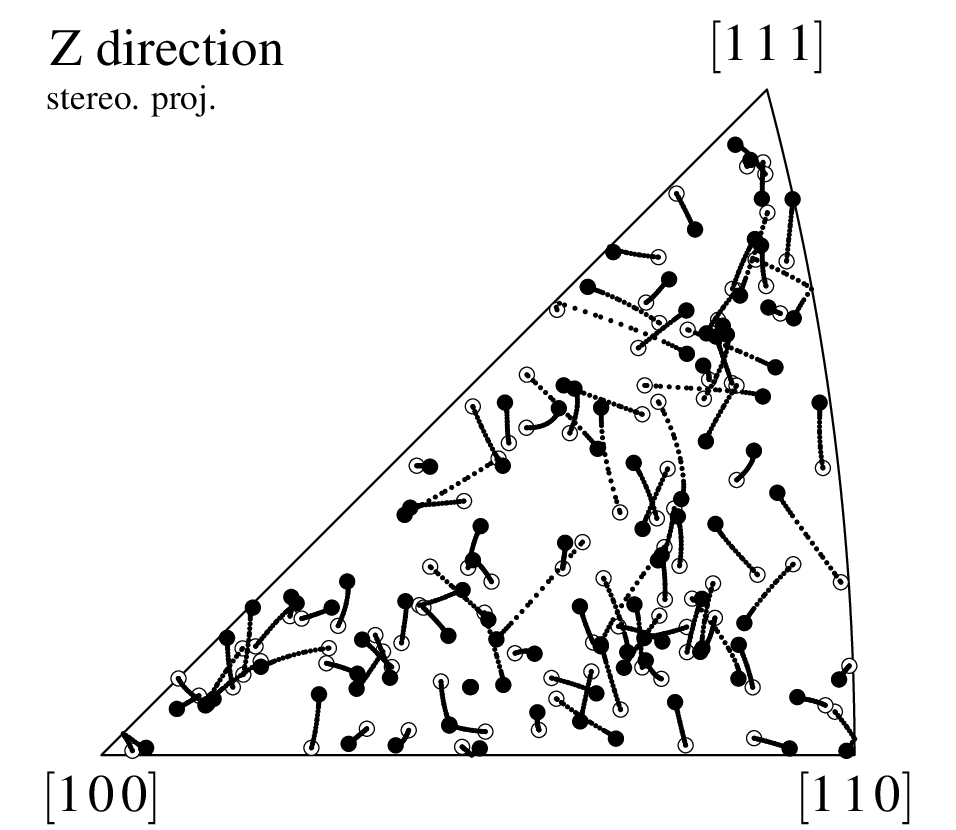
\includegraphics[width=\widF]{figures/testing_fig.png}}
%
\newcommand{\eTimesOTF}[2]{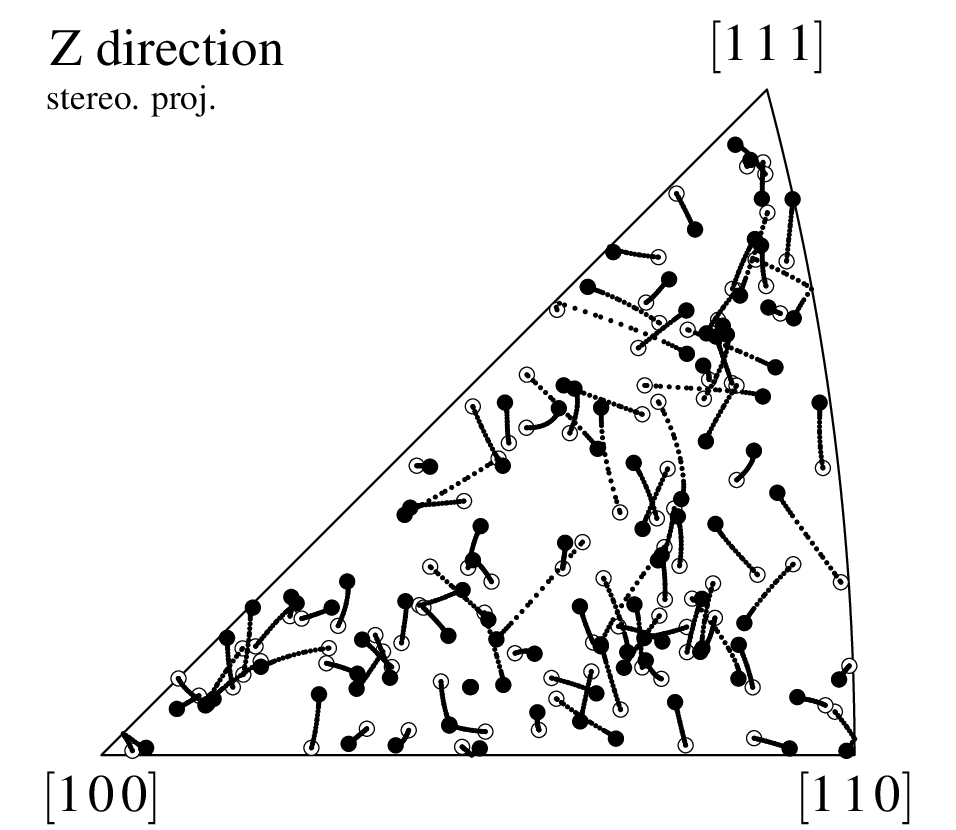
\includegraphics[width=\widF]{figures/testing_fig.png}}
\newcommand{\eTimesOFO}[2]{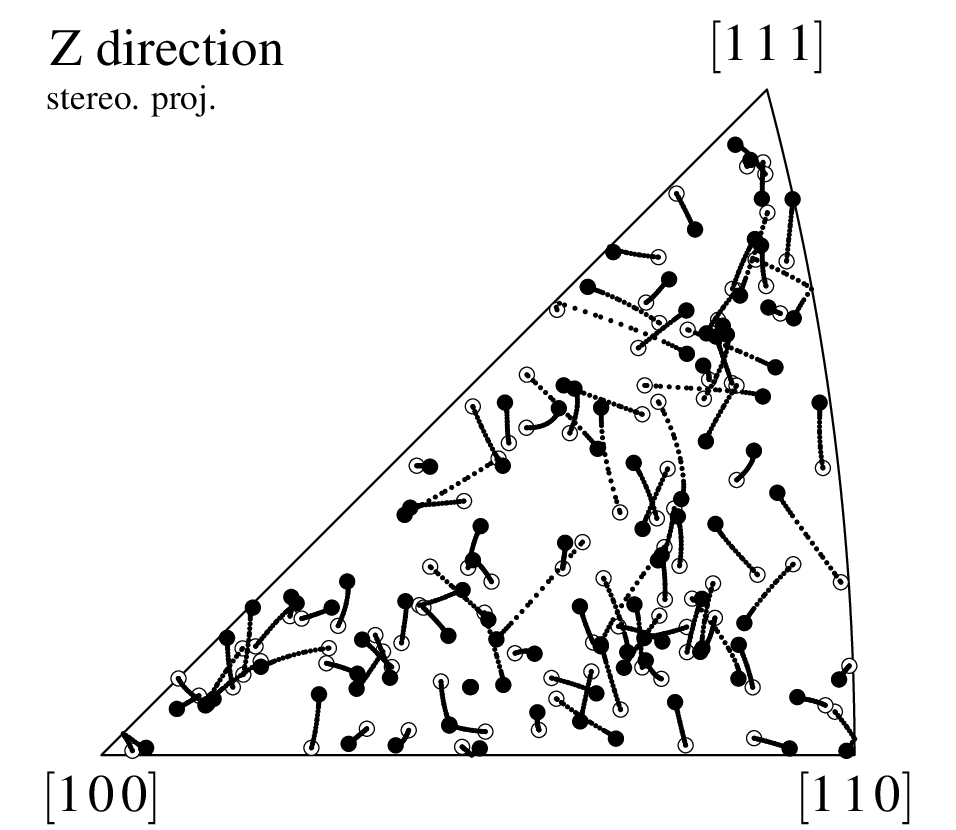
\includegraphics[width=\widF]{figures/testing_fig.png}}
\newcommand{\eTimesOSF}[2]{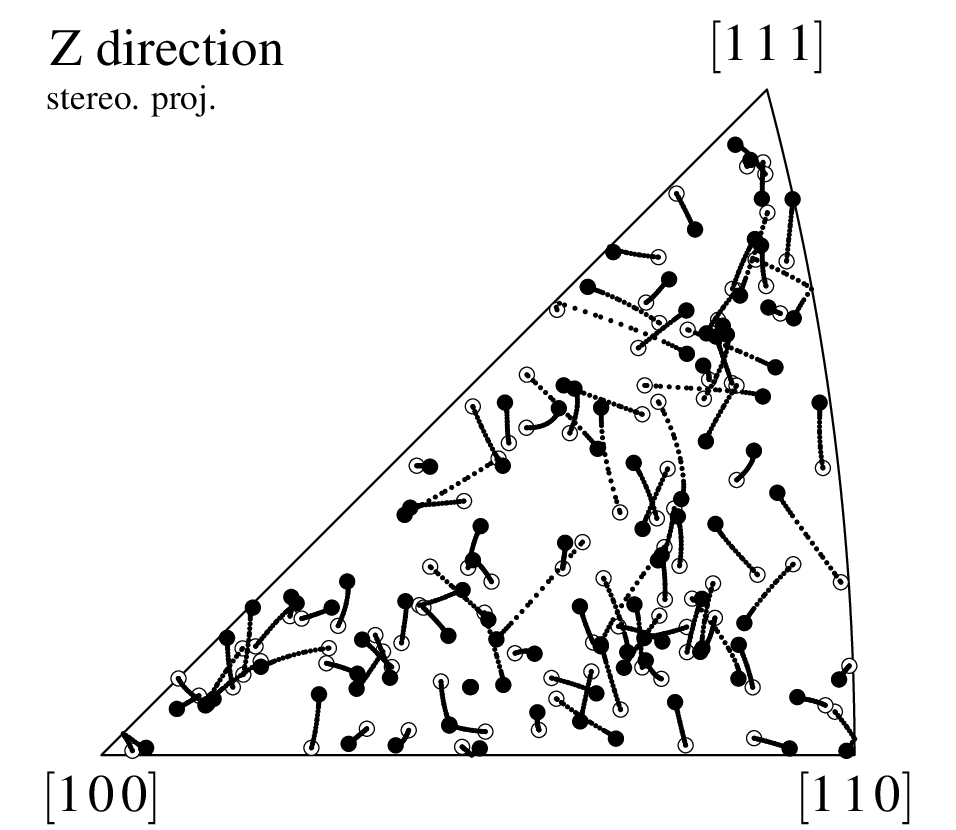
\includegraphics[width=\widF]{figures/testing_fig.png}}
\newcommand{\eTimesTH }[2]{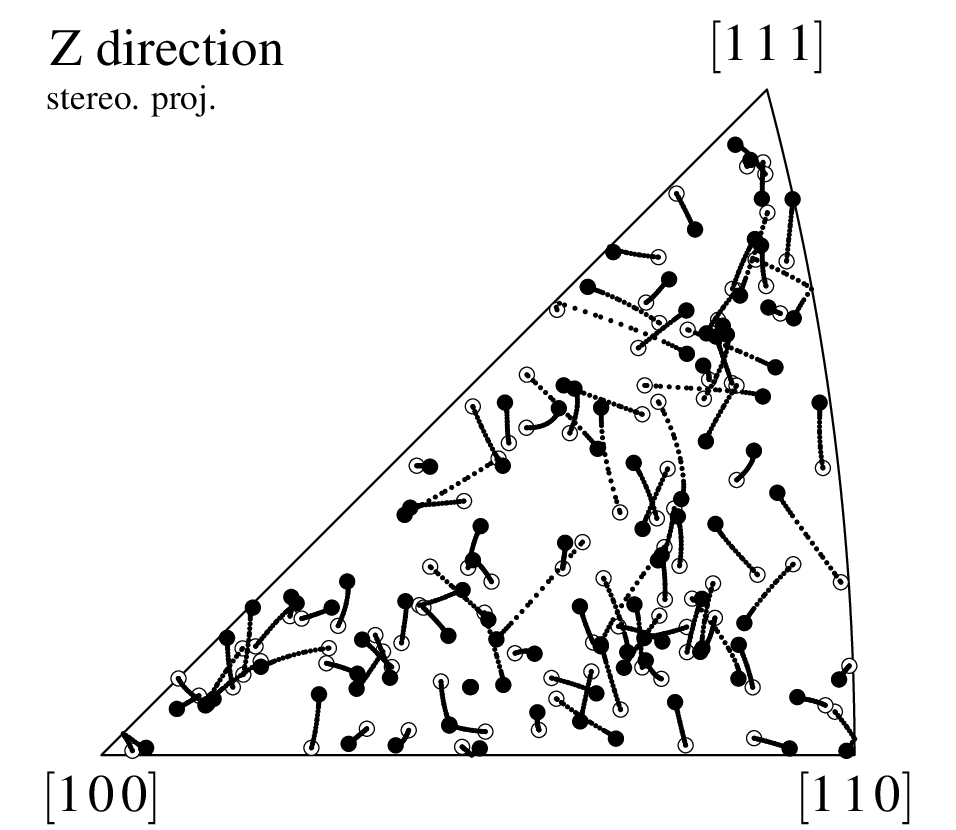
\includegraphics[width=\widF]{figures/testing_fig.png}}
\newcommand{\eTimesFH }[2]{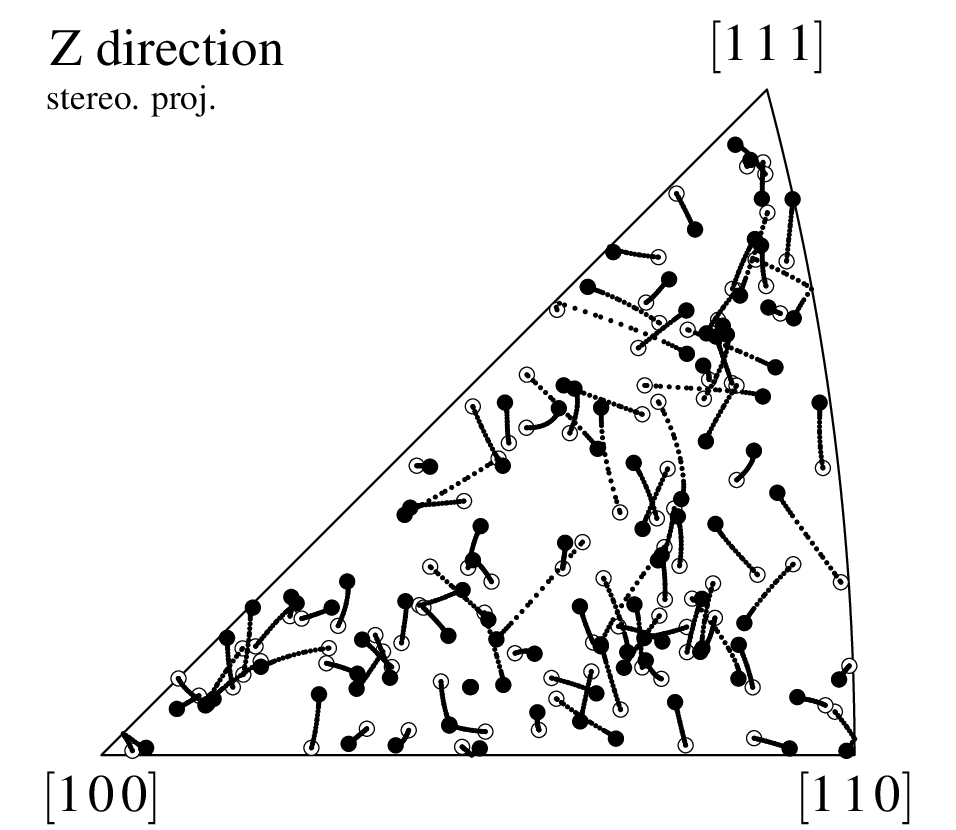
\includegraphics[width=\widF]{figures/testing_fig.png}}
%
\newcommand{\tablee}[1]{ 
\scriptsize{
    \begin{tabular}{|c|c|c|c|c|c|c|c|c|c|c|c|c|}
        \hline
        Simulation &$\hkl(0 1 -1)$ $\hkl[1 1 1]$   &$\hkl(1 0 -1)$ $\hkl[1 1 1]$   &$\hkl(1 -1 0)$ $\hkl[1 1 1]$   &$\hkl(0 1 1)$  $\hkl[1 1 -1]$  &$\hkl(1 0 1)$  $\hkl[1 1 -1]$  &$\hkl(1 -1 0)$ $\hkl[1 1 -1]$  &$\hkl(0 1 1)$  $\hkl[1 -1 1]$  & $\hkl(1 0 -1)$ $\hkl[1 -1 1]$  &$\hkl(1 1 0)$  $\hkl[1 -1 1]$  &$\hkl(0 1 -1)$ $\hkl[1 -1 -1]$ &$\hkl(1 0 1)$  $\hkl[1 -1 -1]$ &$\hkl(1 0 1)$  $\hkl[1 -1 -1]$ \\ \hline \hline
        %\hline
        %&0&1&2&3&4&5&6&7&8&9&10&11\\
         Strength #    & 39.0    & 39.0    & 39.0    & 39.0& 39.0   & 39.0     & 39.0    & 39.     0& 39.0     & 39.0   & 39.0    & 39.0    \\ \hline             
    \end{tabular}}
}
%
\newcommand{\simulation}[3]{
\begin{frame}{Simset number #3}
    \begin{table}[]
        \centering
        \begin{tabular}{|c|ccccc|} 
        \hline
        Domain & 125\% & 150\% & 175\% & 200\% & 400\% &
        \hline
             \polycube&      \cTimesOTF{#1}{#2}& \cTimesOFO{#1}{#2}& \cTimesOSF{#1}{#2}& \cTimesTH{#1}{#2}& \cTimesFH{#1}{#2} \\
             \hline
             \polyelongated& \eTimesOTF{#1}{#2}& \eTimesOFO{#1}{#2}& \eTimesOSF{#1}{#2}& \eTimesTH{#1}{#2}& \eTimesFH{#1}{#2}\\
            \hline
        \end{tabular}
        \label{tab:my_label}
    \end{table}
    \tablee{#3}
\end{frame}

}
% if sim set number <= 25 #1=2, 4 if 25<=simnum<=50 6 if <=75
% #2 = sim setnumber/25 mod 5

\simulation{2}{1}{001-005}
\simulation{1}{1}{005-010}
